\chapter{Methodology}

\section{Simulating the Spin $\frac {1} {2} $ XY Model }
Within this project the spin $\frac{1}{2}$ model is simulated using Python 2.7.
This choice was made primarily due to personal familiarity with the language, as well as the large range of libraries suited to this kind of programming. When I initially started this project the first couple of iterations of code used only the standard Python libraries and Numpy. Due to the exponential scaling of the Hilbert space dimensions of the system and poorly constructed quantitative methods for calculating certain values this scaled extremely poorly with system size. This challenge had numerous solutions which I explored throughout the extent of this project. 

\subsection{Conserved Magnetization Subspace and Reducing Hilbert Space Dimension}
The first problem I reached was the size of the Hamiltonian as a numpy array.
originally attempting to store the full Hamiltonian in a numpy array reaches memory limits relatively quickly, with the Hilbert space scaling $Dim(\mathcal{H}) = 2^N $ where N is the chain length, the array will be of size $2^N,2^N$, if we assume numpy stores a complex number as 2 floats which in python are each 8 bytes, the hamiltonian alone for a system of length $N=16$ would require $\approx$ 67 GB of RAM to store. This is clearly a problem that requires solving such that the system is runnable. 
The first approach to this is to reduce the Hilbert space by creating a conserved magnetization basis, throughout this project we deal almost exclusively with the half filled basis of the Hamiltonian. This alone reduces the system size significantly as seen in figure \ref{fig:fig_HilbertDims}. This alone allows for system sizes of upwards of 16 qubits to be simulated.\\
\begin{figure}
	\centering
	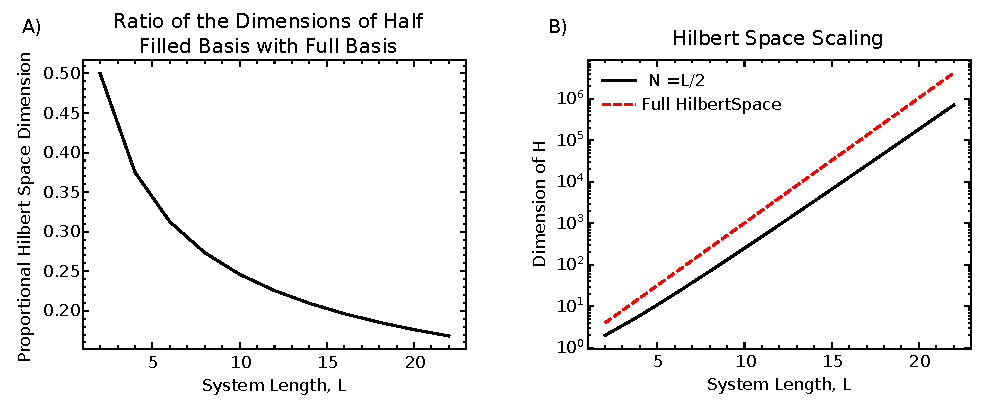
\includegraphics[width=0.75\linewidth]{ratiodims_comp.pdf}
	\caption{Scaling of Hilbert space dimensions. \textbf{A,} The ratio of Hilbert space dimension between the half filled basis and the full hilbert space of a qubit chain of length L. \textbf{B,} showing the exponential increase of the Hilbert space dimension with system size.}
	\label{fig:fig_HilbertDims}
\end{figure}

Another simple implementation that can significantly reduce the memory requirements for constructing a Hamiltonian is the concept of a sparse matrix, as opposed to initiating a matrix with empty values in all of the possible matrix elements, each matrix element is stored in 3 parts; the value in the element, and the corresponding position in the rows and columns. These sparse matrices require significantly less memory to store, however they require slightly special handling in terms of using them in calculations. Two of the main Python modules for scientific computing are Numpy\cite{Numpy}, and SciPy\cite{Scipy} these both have sparse functionality, throughout my work scipy was mainly used for its wider range of functions. 
Although the memory saving is useful sparse matrices encounter problems with certain functions which require rebuilding the full matrix from the sparsely stored version before it can be calculated. Therefore you could store significantly larger matrices however calculating with them still proves challenging. For example the exponentiation of the Hamiltonian to produce the time evolution operator requires the full array, and the sparse variations in Numpy and Scipy simply produce the full array and then act with their exponentiation algorithm.


\subsection{Quantum Python Libraries}
Although this approach was possible and I produced functioning code it wasn't very efficient. This made producing and verifying results extremely time expensive, having spent a large amount of time attempting to improve this myself I turned my attention to pre-existing python libraries which should simplify some portions of the programming.
In the end I used a mixture of two different libraries: Qutip - Quantum Toolkit for python\cite{QUTIP}, and Quspin a library designed for the simulation of quantum many body systems and their exact diagonalization\cite{QUSPIN}. Both of these libraries include significant speed ups over the code that I produced. Part of this is through the implementation of Cython to run certain common equations using C, as well as multi threading where possible. 
Each of these programs have their advantages, Qutip is a more commonly used library however the wide range of potential applications makes certain implementations that were required for this project slightly more intricate to implement. Therefore after a while I explored the QuSpin library which was more explicitly created with the idea of quantum many body dynamics, allowing for easier implementation of many body problems. 

\subsection{Constructing the Hamiltonian}
In order to construct the Hamiltonian we first need to consider the half filled basis. We consider each basis state as a string of zeroes and ones representing the spin up and spin down states, therefore the full basis is trivial to construct. The half filled basis however requires slightly more care. There is no trivial method to calculating the integer values of the binary numbers that have exactly L/2 zeroes within the string, Therefore we simply iterate through the full basis and check each individual string counting the occurrence of zero matches L/2. Using this it is possible to construct a mapping operator that moves between the half filled and full basis. This process is simplified within Quspin, which has its own basis generating functions which allow for simply defining the magnetization subspace symmetry that you want to generate. 

To construct the matrix representation for the Hamiltonian for the XY model \ref{eq:eff_hamiltonian} we simply act the Hamiltonian on each of the basis states and find the respective output. That is the matrix element $\hat{\mathcal{H}}_{ij} = \mel*{i}{\hat{\mathcal{H}}}{j}$ allows us to find the matrix elements for the Hamiltonian. 

\subsubsection{Using Quspin to construct Hamiltonian}

The effective Hamiltonian of the spin $\frac 1 2 $ XY model \ref{eq:eff_hamiltonian} is in that form an integrable model. Therefore in order to observe quantum many body scar effects we must break that integrability. In the paper by Zhang et al.\citep{zhang_many-body_2022} the integrability is broken by the cross coupling terms which come from the physical layout of the device. Therefore it is critical that we add a perturbation to the Hamiltonian such that the integrability is broken. 
Zhang et al\citep{zhang_many-body_2022} use a next-next-nearest neighbour coupling in order to break the integrability of the system for their numerics, we will later explore the impact of changing this, as well as a stepping function in order to speed up thermalization from random states whilst maintaining the dynamics of the pure dimerized states. \\
Using Quspin we initialize a 1D spin $\frac 1 2$ basis, with the $\sum_i^l\hat{S}^z_i = 0 $ where $\hat{S }i^z$ is the Pauli Z spin operator acting on site i. 

we then construct a Hamiltonian of the form 
\begin{equation}
\hat{\mathcal{H}} = \hat{\mathcal{H}}_{1} + \hat{\mathcal{H}}_{2} +\hat{\mathcal{H}}_3
\end{equation}\
where $\hat{\mathcal{H}}_{1}$ is the nearest neighbour interaction \ref{NNHamiltonian}, $\hat{\mathcal{H}}_{2}$ is the next-next nearest interaction \ref{NNNHamiltonian}, and $\hat{\mathcal{H}}_{2}$ is the step function described above \ref{selfhamiltonian}.
\begin{equation} \label{NNHamiltonian}
\hat{\mathcal{H}}_1 = J_a \sum_{i\in Even}^{L-1} ( \hat{S}^+_i\hat{S}^-_{i+1} +\hat{S}^-_i\hat{S}^+_{i+1})  + J_e \sum_{i\in Odd}^{L -1} (\hat{S}^+_i\hat{S}^-_{i+1} +\hat{S}^-_i\hat{S}^+_{i+1})
\end{equation}
where $J_a, J_e$ refer to the intra-dimer and inter-dimer couplings respectively, this alternating coupling strengths are what cause this model to be a representation of the SSH model describe in section \ref{sec:xymodel}.

\begin{equation} \label{NNNHamiltonian}
\hat{\mathcal{H}}_2 = J_{nnn} \sum_{i}^{L-3} ( \hat{S}^+_i\hat{S}^-_{i+3} +\hat{S}^-_i\hat{S}^+_{i+3})
\end{equation}
$ J_{nnn}$ is a constant that describes the next-next-nearest neighbour coupling. This is required to break the integrability of the XY model.

\begin{equation} \label{selfhamiltonian}
\hat{\mathcal{H}}_3 = \sum_i^L \Omega \hat{S}^+\hat{S}^-
\end{equation}
The $\hat{\mathcal{H}}_{3}$ term relates to a transition frequency acting on all sites. As previously described this matrix is stored as a sparse matrix in order to save on memory. This is the default for Hamiltonians in Quspin so requires no additional programming. 

\subsection{Time Evolution}
In order to analyse the dynamics of the system we must calculate the time evolution of this Hamiltonian from varying initial states. One of the states that we will use is the $\ket{\Pi}=\ket{10011001...}$ state. This state is chosen due to it being an experimentally preparable state showing scarred dynamics. 

We will use the Schrodinger equation in order to probe the time evolution of the Hamiltonian. 
\begin{equation}
\label{eq:Schrodinger}
\ket{\psi(t)} = e^{\frac{-i}{\hbar} \hat{H}t}\ket{\psi(0)}
\end{equation}


\section{Quantum Scarring Phenomena}
After constructing the dynamics of the system we will start by looking at some of the common metrics of QMBS, the first of which is the fidelity or overlap. This is measured between $\ket{\psi(0)}$ and $\ket{\psi(t)}$.
This is the one of the observables that shows the periodic revival for the QMBS states. The fidelity is calculated as 
\begin{equation}\label{eq:fidelity}
\mathcal{F} = |\bra{\psi(0)}\ket{\psi(t)}|^2
\end{equation}